\section{Merging of Datasets}

Following curation of individual datasets, these will need to be merged to homogenise variant calls across all data, and generate a square matrix of variant calls, where the union of variants across all samples is available for each population. In order to do this, a union set of calls will be generated for variants that have passed filtering in each dataset (Figure 1). These sites will then be recalled in each dataset to generate genotype likelihoods at these sites. Following this, genotype refinement will be carried out using Beagle v4. For data with pedigree information, this information will be utilised in calling as well as phasing of data. Following refinement of genotype probabilities in Beagle, haplotype phasing will be carried out with SHAPEIT2 to maximise phasing accuracy, especially given the relatedness among some sample sets. MVNcall\cite{Menelaou2013} will then be applied where genotype information is available, within and outside pedigrees to further refine genotype calls based on generating a haplotype scaffold from the 2.5M Omni genotype data available on many sample sets. A possible workflow parallelising data curation across institutions is detailed in Appendix 1. 

\begin{figure}[h]
\caption{Homogenised calling across all datasets to generate a single panel}
\centering
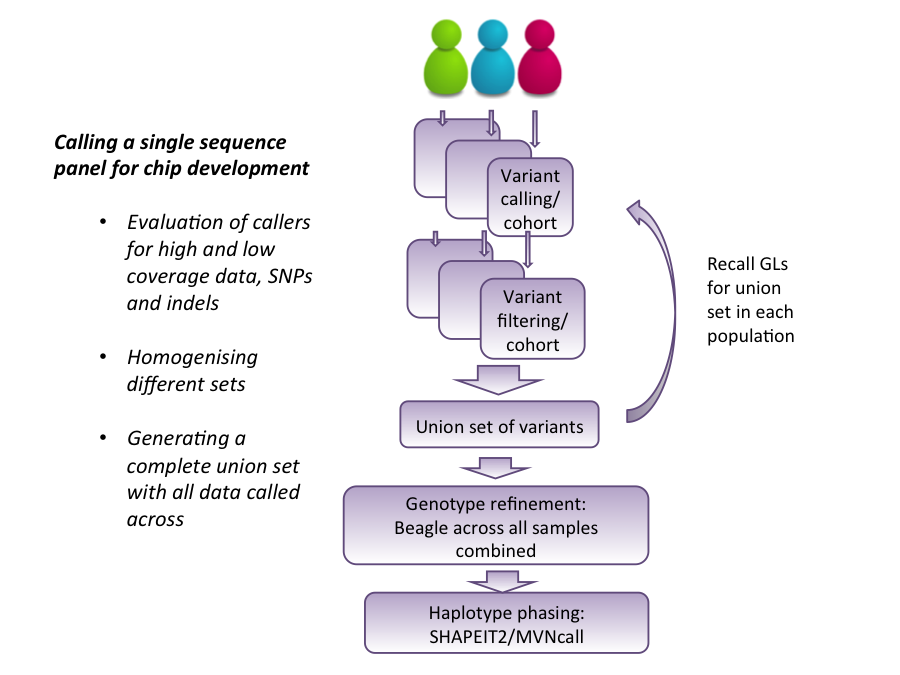
\includegraphics[width=0.5\textwidth]{calling}
\end{figure}
